\chapter{Modelling of the Vehicle}\label{cha:ModelOfVehicle}

\begin{figure}[H]
	\centering
	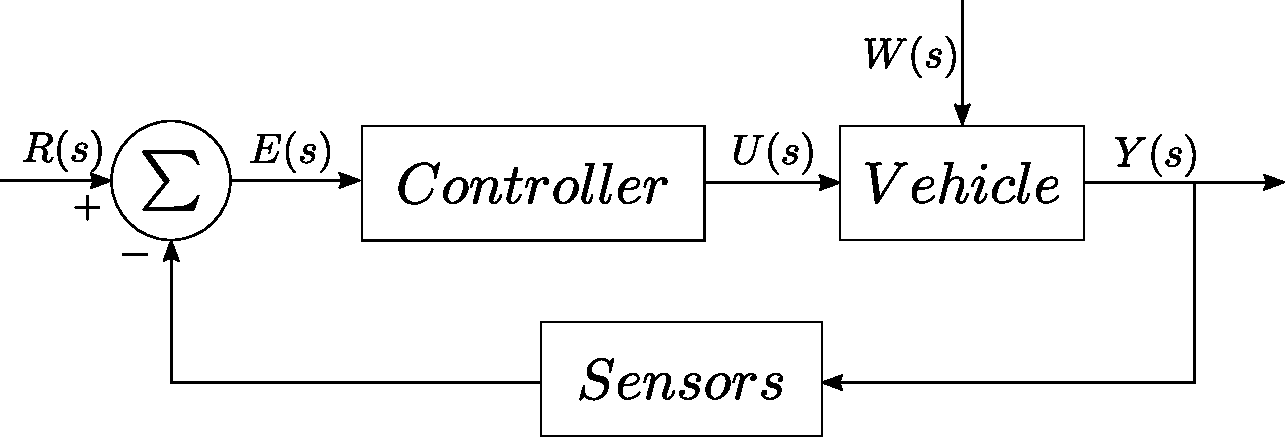
\includegraphics[scale=0.6]{figures/StartTotalModelsystem.pdf}
	\caption{A block diagram of the velocity model}
	\label{fig:StartTotalModelsystem}
\end{figure}

The input in the velocity model, $R(s)$, is the vehicles wanted velocity and the output is the actual velocity of the vehicle. The controller receives an input, $E(s)$, which consist of the wanted speed subtracted with the actual speed measured with a sensor. Hence delivering a error which to be corrected to be able to achieve the wanted speed as an output. The controller should therefore deliver a voltage to the Vehicle, $U(s)$, thus, changing the rotational force of the motor and thereby change the vehicles velocity. The vehicle is also affected by a external disturbance, $W(s)$, e.g. a slope, wind or ground friction. The vehicles output, $Y(s)$ is the actual velocity of the vehicle. The actual velocity is measured by the sensors and subtracted from the wanted speed.